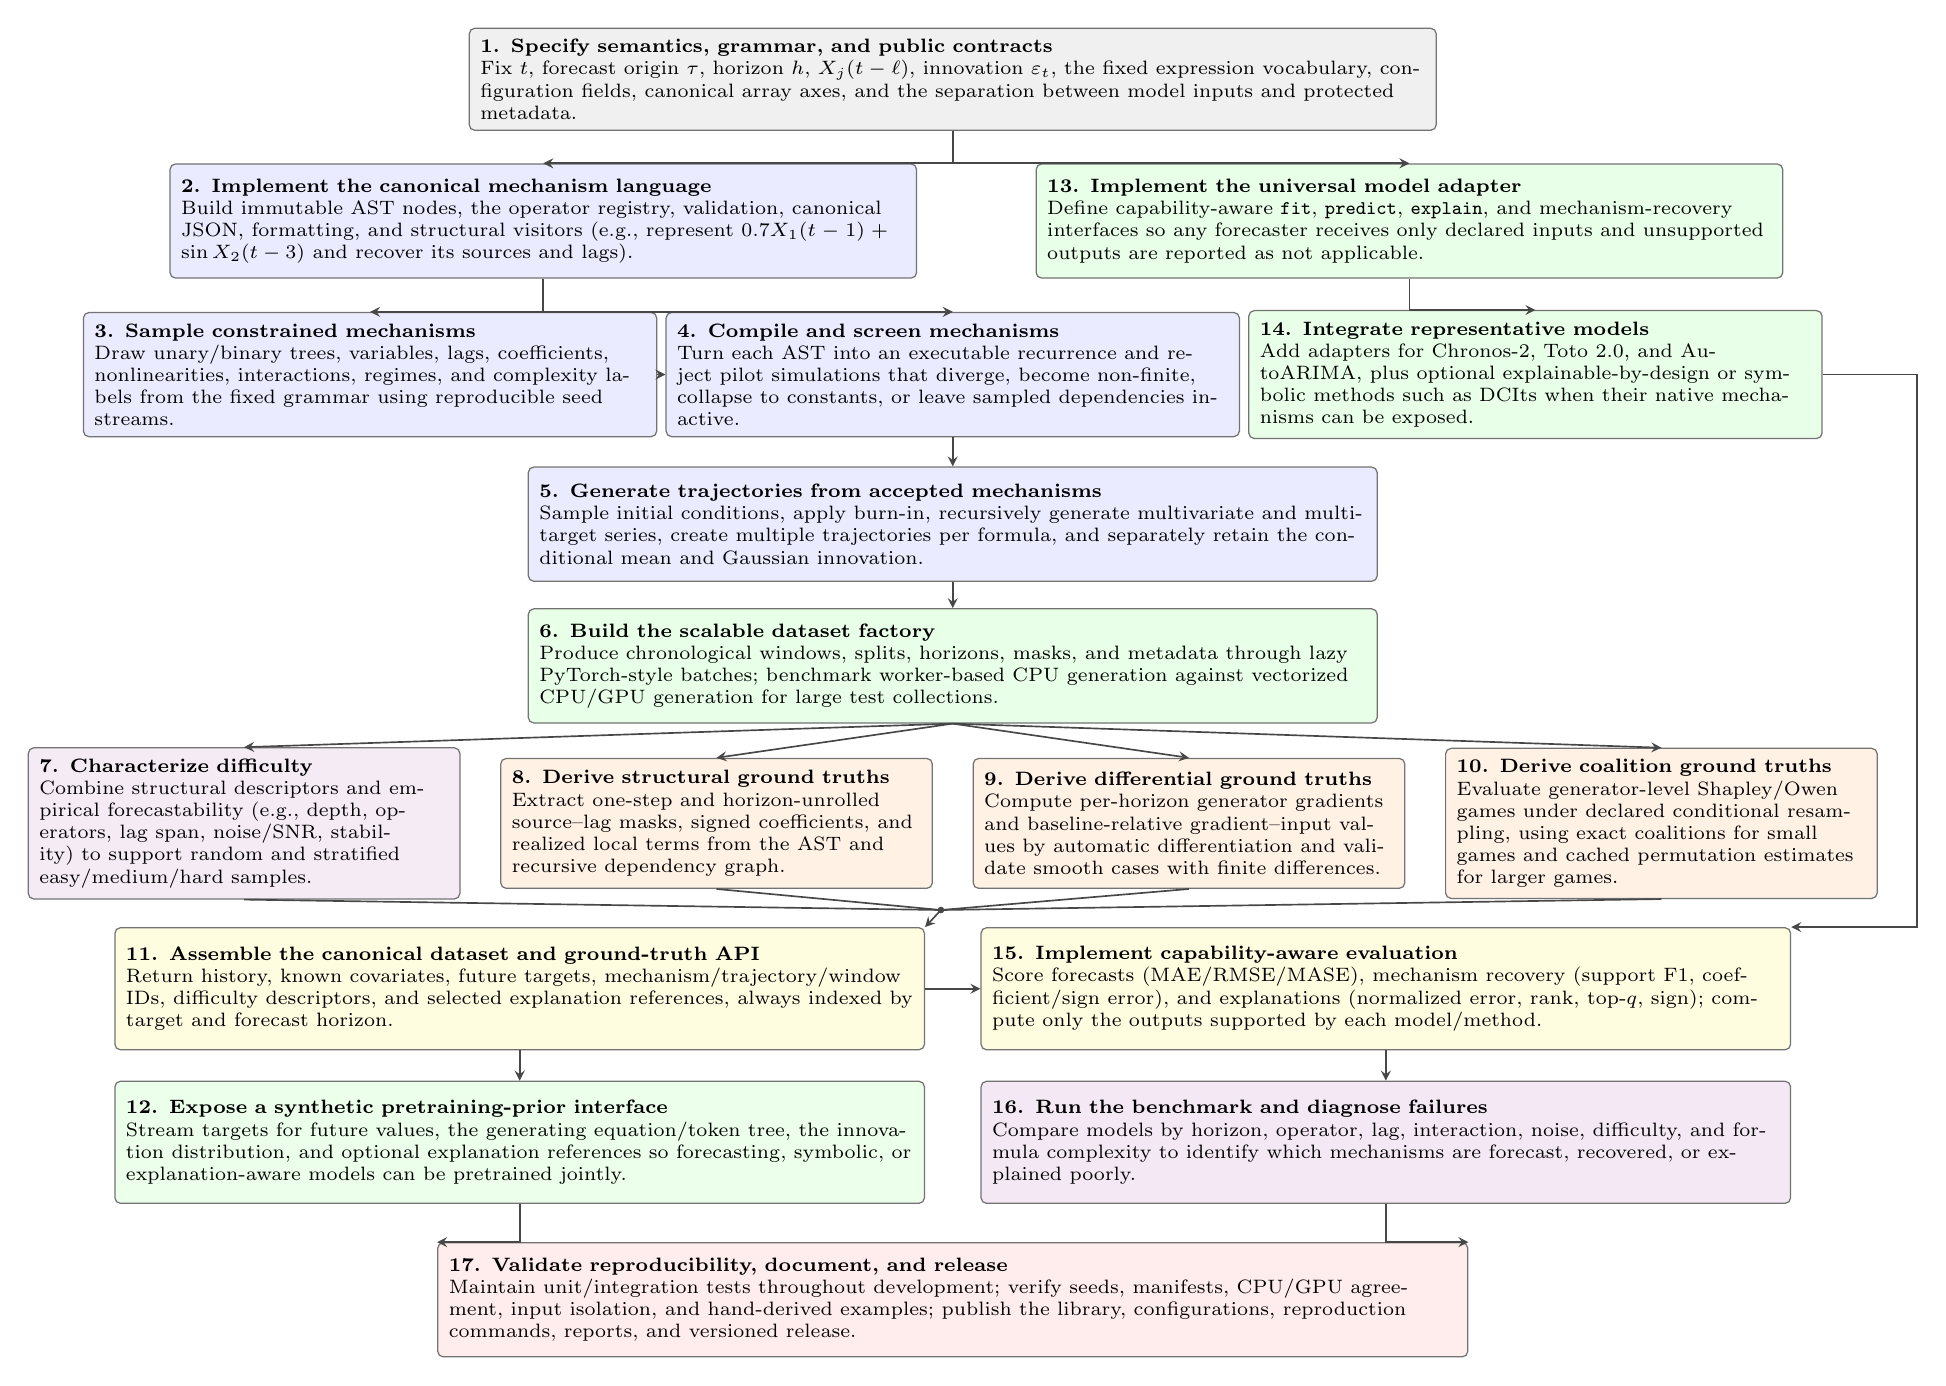
\begin{tikzpicture}[
    x=1cm,
    y=1cm,
    task/.style={
        draw=black!55,
        line width=0.45pt,
        rounded corners=2pt,
        align=left,
        inner sep=4pt,
        font=\scriptsize
    },
    dependency/.style={->,>=stealth,semithick,draw=black!72},
    joinline/.style={semithick,draw=black!72}
]

% Shared scientific and software foundation.
\node[task,fill=black!6,text width=12.0cm,minimum height=1.25cm] (specification) at (0,7.4) {%
    \textbf{1. Specify semantics, grammar, and public contracts}\par
    Fix $t$, forecast origin $\tau$, horizon $h$, $X_j(t-\ell)$, innovation
    $\varepsilon_t$, the fixed expression vocabulary, configuration fields,
    canonical array axes, and the separation between model inputs and protected metadata.
};

\node[task,fill=blue!8,text width=9.2cm,minimum height=1.45cm] (language) at (-5.2,5.6) {%
    \textbf{2. Implement the canonical mechanism language}\par
    Build immutable AST nodes, the operator registry, validation, canonical JSON,
    formatting, and structural visitors (e.g., represent
    $0.7X_1(t-1)+\sin X_2(t-3)$ and recover its sources and lags).
};

% The adapter boundary can start from the public contracts while generators are built.
\node[task,fill=green!9,text width=9.2cm,minimum height=1.45cm] (adapter) at (5.8,5.6) {%
    \textbf{13. Implement the universal model adapter}\par
    Define capability-aware \texttt{fit}, \texttt{predict}, \texttt{explain}, and
    mechanism-recovery interfaces so any forecaster receives only declared inputs and
    unsupported outputs are reported as not applicable.
};

\node[task,fill=blue!8,text width=7.0cm,minimum height=1.55cm] (sampler) at (-7.4,3.65) {%
    \textbf{3. Sample constrained mechanisms}\par
    Draw unary/binary trees, variables, lags, coefficients, nonlinearities,
    interactions, regimes, and complexity labels from the fixed grammar using
    reproducible seed streams.
};

\node[task,fill=blue!8,text width=7.0cm,minimum height=1.55cm] (compiler) at (0,3.65) {%
    \textbf{4. Compile and screen mechanisms}\par
    Turn each AST into an executable recurrence and reject pilot simulations that
    diverge, become non-finite, collapse to constants, or leave sampled dependencies
    inactive.
};

\node[task,fill=green!9,text width=7.0cm,minimum height=1.55cm] (models) at (7.4,3.65) {%
    \textbf{14. Integrate representative models}\par
    Add adapters for Chronos-2, Toto~2.0, and AutoARIMA, plus optional
    explainable-by-design or symbolic methods such as DCIts when their native
    mechanisms can be exposed.
};

\node[task,fill=blue!8,text width=10.5cm,minimum height=1.45cm] (trajectories) at (0,1.75) {%
    \textbf{5. Generate trajectories from accepted mechanisms}\par
    Sample initial conditions, apply burn-in, recursively generate multivariate and
    multi-target series, create multiple trajectories per formula, and separately
    retain the conditional mean and Gaussian innovation.
};

\node[task,fill=green!9,text width=10.5cm,minimum height=1.45cm] (dataset) at (0,-0.05) {%
    \textbf{6. Build the scalable dataset factory}\par
    Produce chronological windows, splits, horizons, masks, and metadata through lazy
    PyTorch-style batches; benchmark worker-based CPU generation against vectorized
    CPU/GPU generation for large test collections.
};

% Parallel products derived from the retained mechanism and generated observations.
\node[task,fill=violet!8,text width=5.2cm,minimum height=1.65cm] (difficulty) at (-9.0,-2.05) {%
    \textbf{7. Characterize difficulty}\par
    Combine structural descriptors and empirical forecastability (e.g., depth,
    operators, lag span, noise/SNR, stability) to support random and stratified
    easy/medium/hard samples.
};

\node[task,fill=orange!10,text width=5.2cm,minimum height=1.65cm] (structural) at (-3.0,-2.05) {%
    \textbf{8. Derive structural ground truths}\par
    Extract one-step and horizon-unrolled source--lag masks, signed coefficients, and
    realized local terms from the AST and recursive dependency graph.
};

\node[task,fill=orange!10,text width=5.2cm,minimum height=1.65cm] (gradient) at (3.0,-2.05) {%
    \textbf{9. Derive differential ground truths}\par
    Compute per-horizon generator gradients and baseline-relative gradient--input
    values by automatic differentiation and validate smooth cases with finite
    differences.
};

\node[task,fill=orange!10,text width=5.2cm,minimum height=1.65cm] (coalition) at (9.0,-2.05) {%
    \textbf{10. Derive coalition ground truths}\par
    Evaluate generator-level Shapley/Owen games under declared conditional resampling,
    using exact coalitions for small games and cached permutation estimates for larger
    games.
};

\node[task,fill=yellow!12,text width=10.0cm,minimum height=1.55cm] (canonicalapi) at (-5.5,-4.15) {%
    \textbf{11. Assemble the canonical dataset and ground-truth API}\par
    Return history, known covariates, future targets, mechanism/trajectory/window IDs,
    difficulty descriptors, and selected explanation references, always indexed by
    target and forecast horizon.
};

\node[task,fill=yellow!12,text width=10.0cm,minimum height=1.55cm] (evaluation) at (5.5,-4.15) {%
    \textbf{15. Implement capability-aware evaluation}\par
    Score forecasts (MAE/RMSE/MASE), mechanism recovery (support F1, coefficient/sign
    error), and explanations (normalized error, rank, top-$q$, sign); compute only the
    outputs supported by each model/method.
};

% Two intended uses of the generated data and ground truths.
\node[task,fill=green!8,text width=10.0cm,minimum height=1.55cm] (prior) at (-5.5,-6.10) {%
    \textbf{12. Expose a synthetic pretraining-prior interface}\par
    Stream targets for future values, the generating equation/token tree, the
    innovation distribution, and optional explanation references so forecasting,
    symbolic, or explanation-aware models can be pretrained jointly.
};

\node[task,fill=violet!9,text width=10.0cm,minimum height=1.55cm] (benchmark) at (5.5,-6.10) {%
    \textbf{16. Run the benchmark and diagnose failures}\par
    Compare models by horizon, operator, lag, interaction, noise, difficulty, and
    formula complexity to identify which mechanisms are forecast, recovered, or
    explained poorly.
};

\node[task,fill=red!7,text width=12.8cm,minimum height=1.45cm] (release) at (0,-8.10) {%
    \textbf{17. Validate reproducibility, document, and release}\par
    Maintain unit/integration tests throughout development; verify seeds, manifests,
    CPU/GPU agreement, input isolation, and hand-derived examples; publish the library,
    configurations, reproduction commands, reports, and versioned release.
};

% Hard technical dependencies.
\draw[dependency] (specification.south) -- ++(0,-0.22) |- (language.north);
\draw[dependency] (specification.south) -- ++(0,-0.22) |- (adapter.north);

\draw[dependency] (language.south) -- ++(0,-0.22) |- (sampler.north);
\draw[dependency] (language.south) -- ++(0,-0.22) |- (compiler.north);
\draw[dependency] (sampler.east) -- (compiler.west);
\draw[dependency] (compiler.south) -- (trajectories.north);
\draw[dependency] (trajectories.south) -- (dataset.north);

\draw[dependency] (adapter.south) -- ++(0,-0.22) |- (models.north);

\draw[dependency] (dataset.south) -- (difficulty.north);
\draw[dependency] (dataset.south) -- (structural.north);
\draw[dependency] (dataset.south) -- (gradient.north);
\draw[dependency] (dataset.south) -- (coalition.north);

\coordinate (productjoin) at (-0.15,-3.15);
\draw[joinline] (difficulty.south) -- (productjoin);
\draw[joinline] (structural.south) -- (productjoin);
\draw[joinline] (gradient.south) -- (productjoin);
\draw[joinline] (coalition.south) -- (productjoin);
\fill[black!72] (productjoin) circle (1.2pt);
\draw[dependency] (productjoin) -- (canonicalapi.north east);

\draw[dependency] (canonicalapi.south) -- (prior.north);
\draw[dependency] (canonicalapi.east) -- (evaluation.west);
\draw[dependency] (models.east) -- ++(1.2,0) |- (evaluation.north east);
\draw[dependency] (evaluation.south) -- (benchmark.north);

\draw[dependency] (prior.south) -- ++(0,-0.22) |- (release.north west);
\draw[dependency] (benchmark.south) -- ++(0,-0.22) |- (release.north east);

\end{tikzpicture}
